\documentclass[10pt,twocolumn]{article} 

\usepackage{oxycomps} % use the main oxycomps style file

\bibliography{references}

\pdfinfo{
    /Title (Writing Your Oxy CS Comps Paper in LaTeX)
    /Author (Justin Li)
}

\title{Writing Your Oxy CS Comps Paper in \LaTeX}

\author{Justin Li}
\affiliation{Occidental College}
\email{justinnhli@oxy.edu}

\begin{document}

\maketitle

\begin{abstract}
    This document serves as an introduction to {\LaTeX} and also describes the requirements of the senior project final paper for Occidental College's Computer Science majors.
    We start by justifying the use of {\LaTeX} over Word, Google Docs, and other What-You-See-Is-What-You-Get (WYSISYG) editors.
    A brief tutorial to {\LaTeX} follows, reviewing the most common commands and environments used in technical papers.
    We then turn our attention to the Oxy CS Comps Paper, first contextualizing it within the major curriculum, before exploring each major section of the paper in detail.
    We conclude with some miscellaneous tips for successfully completing comps.
\end{abstract}

\section{Introduction}

\section{Using \LaTeX}

LaTeX (pronounced \textit{lah-teck} or \textit{lay-teck}), often stylized as {\LaTeX} and written as latex, is a document markup language and typesetting system.
Building on the {\TeX} language created by Donald Knuth in 1978, LaTeX provides additional commands for common document needs such as sections, figures, and bibliographies.
LaTeX is widely used in academia, especially in mathematical fields, due to how easy it is to write mathematical equations and its automatic management of references.
Since it is a markup language, LaTeX source files are written in plain text, which also makes it compatible with version control systems like git.

The most primitive syntax of LaTeX is the \textit{macro} or \textit{command}, which is always written with a backslash followed by the name of the command.
The {\LaTeX} glyph, for example, can be created with the command \texttt{\textbackslash LaTeX}.
Some commands take parameters, which are denoted in braces (e.g., \texttt{\textbackslash usepackage\{biblatex\}} will import the \texttt{biblatex} package), with some commands additionally accepting options in square brackets (e.g., \texttt{\textbackslash usepackage[style=numeric]\{biblatex\}}).
The \texttt{\textbackslash begin} and \texttt{\textbackslash end} commands are special, as they indicate the start and end of an \textit{environment}.
The content of a LaTeX document, for example, is surrounded by \texttt{\textbackslash begin\{document\}} and \texttt{\textbackslash end\{document\}}, indicating the text that should appear in the document.

\begin{figure}
    \centering
    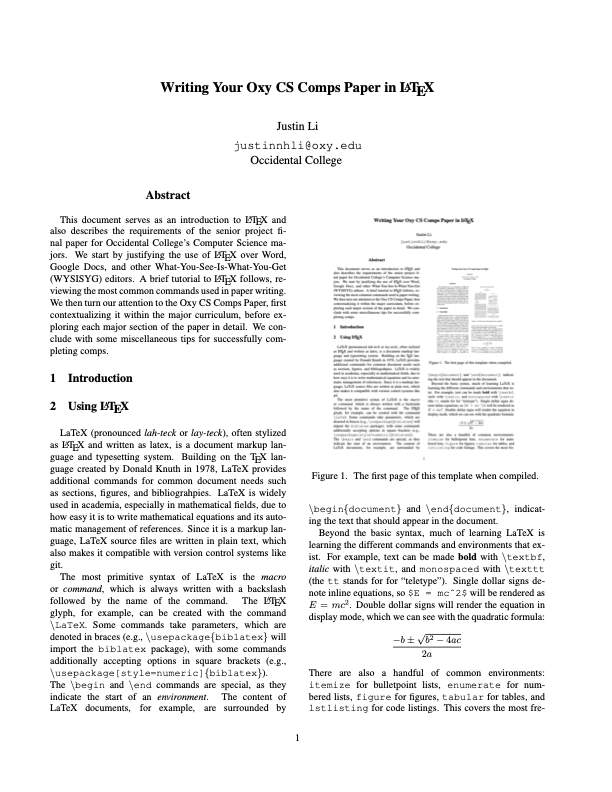
\includegraphics[width=.95\linewidth]{first-page.png}
    \caption{
        The first page of this template when compiled.
    }
    \label{fig:first-page}
\end{figure}

Beyond the basic syntax, much of learning LaTeX is learning the different commands and environments that exist.
For example, text can be made \textbf{bold} with \texttt{\textbackslash textbf}, \textit{italic} with \texttt{\textbackslash textit}, and \texttt{monospaced} with \texttt{\textbackslash texttt} (the \texttt{tt} stands for for ``teletype'').
Single dollar signs denote inline equations, so \texttt{\$E = mc\textasciicircum 2\$} will be rendered as $E = mc^2$.
Double dollar signs will render the equation in display mode, which we can see with the quadratic formula:
$$\frac{{-b \pm \sqrt {b^2 - 4ac} }}{{2a}}$$
There are also a handful of common environments:

\begin{itemize}
    \item \texttt{itemize} for bulletpoint lists
    \item \texttt{enumerate} for numbered lists
    \item \texttt{figure} for figures (see Figure \ref{fig:first-page})
    \item \texttt{tabular} for tables
    \item \texttt{lstlisting} for code listings (see Listing \ref{lst:python-hello-world})
\end{itemize}

\begin{lstlisting}[
    language=Python,
    caption={Hello, World! in Python},
    label={lst:python-hello-world},
    float
]
def hello():
    print('hello, world!')
\end{lstlisting}

This covers the most frequently used commands, but as you might have already inferred, LaTeX is a vast and deep system, and can easily be overwhelming.
We recommended reading through the \citetitle{Overleaf2021LearnLaTeXIn} tutorial \cite{Overleaf2021LearnLaTeXIn} and using the \citetitle{WikiBook2022LaTeX} \cite{WikiBook2022LaTeX} as reference.
Beyond that, you should examine and play with the source of this document to gain working proficiency with LaTeX.

One final note on writing in LaTeX.
Since LaTeX is only a markup language, the source files must be compiled into a viewable form, most commonly into a PDF file.
The source of this document is made up of several files, each with its own purpose:
\begin{itemize}
    \item \texttt{template.tex} - The main LaTeX file containing the contents of the document.
    \item \texttt{oxycomps.sty} - A style file with settings for what the document should look like.
    \item \texttt{references.bib} - A list of bibliography items.
    \item Other files containing images, build instructions, etc.
\end{itemize}
Manual compilation of these files is somewhat esoteric, as it requires multiple uses of the \texttt{pdflatex} and \texttt{biblatex} commands.
Instead, it is much easier to use tools such as \texttt{pdflatex} or \texttt{latexmk} (in the terminal) or Overleaf (online) for compilation.
We have also provided a \texttt{Makefile} which will automatically update the document as necessary; the use of makefiles is beyond the scope of this document, but see \textcite{Lambert2021MakefileTutorial}.

\begin{comment}
No definition citations, unless the term itself is in dispute
Separate problem background from technical background
    Unclear if games and apps require much technical background
    The general structure of the framework might be better suited for the Architecture Overview section
        Eg. Flask uses decorators to associate functions with URLs
        Eg. Unity has scripts associated with objects and specific triggers, such as walking into an area, pressing a button, etc.
    Maybe a better name is "algorithmic background"?
        Should explore what does and doesn't count
            All ML counts
            App and game frameworks do not
        Framework vs. library?
            I like the idea of [inversion of control](https://martinfowler.com/bliki/InversionOfControl.html), but that may be too abstract for students to understand
        Heuristic: is understanding that system necessary to understand the results?
            Ie. How Flask or Unity works doesn't influence whether the app/game is useful/fun/engaging
            But how (say) linear regression works is highly relevant for why the results match/don't match the actual values
\end{comment}

\section{The Oxy CS Comps Paper}

\subsection{Goals}

\subsection{Audience}

\subsection{Requirements}

\section{Sections of the Oxy CS Comps Paper}

\subsection{Introduction and Background}

\subsection{Prior Work}

\subsection{Methods}

\subsection{Evaluation}

\subsection{Ethical Considerations}

\subsection{Limitations, Future Work, and Conclusion}

\subsection{Appendices}

\section{Conclusion}

\printbibliography 

\end{document}
